\documentclass[
 manuscript=article,  %% article (default),SpecialIssue,data,software,editorial
  layout=publish, 
  year=2024, 
  month= Februari, %check cls jika dibutuhkan
  volume=8,
  number=1 
]{JIKO}
\usepackage{hyphenat} 
%%%%++++++++++++++++++++++
\hyphenation{
	soft-ware 										
	di-la-ku-kan 
	di-la-kukan 
	me-nam-bah-kan
	meng-gu-na-kan
}
%%%%++++++++++++++++++++++
\usepackage{algorithm,algpseudocode}
\usepackage{courier,multirow,multicol}
\usepackage{listings}
\usepackage[bahasa,english]{babel}
\usepackage{blindtext}

\lstset{basicstyle=\ttfamily \small , language=python} 
\lstset{basicstyle=\ttfamily \small, language=html}
\lstset{basicstyle=\ttfamily \small, language=c++}

\doi{10.26798/jiko.}

%%%%%%%%%%%%%%%%%%%%%%%%%%%%%%%%%%%%%%%%%%%%%%
%%											%%
%%				RIKIE - UTDI- 				%%
%%											%%
%%%%%%%%%%%%%%%%%%%%%%%%%%%%%%%%%%%%%%%%%%%%%%

\newcommand{\id}{xxx} %Sesuaikan dengan ID Artikel
\setcounter{page}{15}  %Halaman pertama



\frenchspacing

% --- AREA AUTHOR ---
% Pastikan Judul artikel tidak lebih dari 12 kata
\title{%
	Perbandingan Efektivitas Desain User Experience pada Platform Pembayaran Digital (Studi Kasus pada GoPay, OVO, Dana)\\
	% {\large Sub-judul jika diperlukan}\\[1ex]
	\itshape Comparison of the Effectiveness of User Experience Design on Digital Payment Platforms (Case Study on GoPay, OVO and Dana)\\
	% {\large Subtitle if needed in English}%
}

\newcommand{\judul}{Judul Dalam Bahasa Indonesia-Sub-judul jika diperlukan}

\author{Angga Permana}
\email{2110631170049@student.unsika.ac.id} %---> pindahkan email ini dibawah author korespondensi.
\newcommand{\refnama}{M. I. Alharits} %Pastikan ini benar
\affiliation{Informatika, Fakultas Ilmu Komputer, Universitas Singaperbangsa Karawang, Jawa Barat, Indonesia}




% Mkasimum 5 Kata dalam keywords
\keywords{JIKO.cls; \ \LaTeX;Pembayaran Digital; Pengalaman Pengguna; SUS; UEQ} 

\keywordsing{JIKO.cls; \ \LaTeX;Digital Payments; User Experience; SUS; UEQ} 
% Penting, hanya indeks singkatan jika istilah berisi lebih dari dua kata, dan istilah tersebut digunakan lebih dari sepuluh kali di seluruh makalah. Jika tidak, uraikan secara lengkap di dalam artikel.


\begin{document}
%\begin{CJK*}{UTF8}{gbsn}

%%%%%%%%%%%%%% ABSTRAK %%%%%%%%%%%%%%%%%%%%%%%%%%%%
 
\begin{abstract}
\noindent\hspace{0.6cm}  Jumlah masyarakat Indonesia yang menggunakan ponsel pintar terus meningkat setiap tahunnya, sehingga mendorong para pengembang aplikasi untuk terus menciptakan cara baru dan kreatif dalam menawarkan opsi pembayaran digital yang memudahkan pengguna dalam melakukan transaksi non-tunai.  Meskipun banyak aplikasi pembayaran digital lain yang tersedia saat ini GoPay, OVO, dan Dana adalah yang paling banyak digunakan. Tujuan dari penelitian ini adalah untuk membandingkan tiga aplikasi pembayaran digital dengan berbagai proses bisnis dan fitur yang hampir identik dalam hal pengalaman pengguna. Penelitian ini membandingkan analisis pengalaman pengguna berdasarkan kriteria kuesioner pengalaman pengguna dan skala kegunaan sistem. Kuesioner SUS dibagikan kepada 20 responden dan kuesioner UEQ dibagikan kepada 30 responden. Hasil dari kuesioner SUS menunjukan keberhasilan yang cukup tinggi kepada ketiga aplikasi pembayaran digital yang dimana aplikasi dana memiliki nilai lebih baik yaitu 53 sedangkan aplikasi GoPay mendapatkan nilai 50 dan aplikasi ovo mendapatkan nilai 49. Hasil dari kuesioner UEQ responden memiliki kesan yang baik terhadap ketiga aplikasi pembayaran digital tersebut. Aplikasi GoPay memiliki hasil lebih unggul pada lima aspek yaitu Daya tarik, Kejelasan, Efisiensi, Ketepatan dan Stimulasi, sedangkan aplikasi Dana mendapatkan hasil lebih baik dalam satu aspek skala yaitu aspek Kebaruan.
\end{abstract}

\begin{abstracting}
\noindent\hspace{0.6cm}  The number of Indonesians using smartphones continues to increase every year, thus encouraging application developers to continue to create new and creative ways to offer digital payment options that make it easier for users to carry out non-cash transactions. Although there are many other digital payment applications available today, Gopay, OVO and Dana are the most widely used. The aim of this research is to compare three digital payment applications with different business processes and features that are almost identical in terms of user experience. This research compares user experience analysis based on user experience questionnaire criteria and system usability scales. The SUS questionnaire was distributed to 20 respondents and the UEQ questionnaire was distributed to 30 respondents. The results of the SUS questionnaire show quite high success for the three digital payment applications, where the Dana application has a better score, namely 53, while the GoPay application gets a score of 50 and the OVO application gets a score of 49. The results of the UEQ questionnaire, respondents have a good impression of the three payment applications digital. The Gopay application has superior results in five aspects, namely Attractiveness, Clarity, Efficiency, Accuracy and Stimulation, while the Dana application gets better results in one scale aspect, namely the Novelty aspect
\end{abstracting}
%%%%%%%%%%%%%%%%%%%%%%%%%%%% PENDAHULUAN %%%%%%%%%%%%%%%%

\section{Pendahuluan}
% ------ P 1
Saat ini perkembangan teknologi informasi sangat bermanfaat dan berperan penting dalam berbagai industri, khususnya di bidang transaksi pembayaran. Pentingnya uang tunai dalam transaksi pembayaran digital telah digantikan oleh kemajuan teknologi dalam sistem pembayaran. Hal ini diperkuat dengan semakin populernya pusat perbelanjaan dan bisnis yang menerima pembayaran digital. Di Indonesia, ponsel digunakan melalui program pembayaran digital untuk meningkatkan layanan. Dengan penggunaan dompet elektronik, pengguna dapat melakukan transaksi online non-tunai untuk memperoleh produk dan layanan, seperti pembayaran tagihan, pembelian kredit, transfer uang, dan pembayaran pedagang. Salah tiga dari aplikasi pembayaran digital yaitu gopay, ovo dan dana. Berdasarkan penelitian oleh Snapcart pada tahun 2019, yang merupakan lembaga riset berbasis aplikasi, sebanyak 58\% dari 1.800 responden memilih OVO sebagai aplikasi pembayaran digital favorit. GoPay berada di posisi kedua dengan 23\%, diikuti oleh DANA dengan 6\%. Eko Wicaksono, perwakilan Snapcart Indonesia, menjelaskan bahwa pengguna aplikasi pembayaran digital mengapresiasi kemudahan, kecepatan, keamanan, dan efisiensi dalam bertransaksi \cite{1}.
%  ----- P 2
\\ \\ 
Salah satu faktor yang mempengaruhi layanan pembayaran digital itu sendiri adalah penggunaan aplikasi mobile untuk mengetahui keinginan pelanggan, yang pada akhirnya akan menghasilkan kepuasan produk. Oleh karena itu, hal ini memberikan tantangan bagi pengembang aplikasi pembayaran digital untuk terus meningkatkan aplikasinya guna memenuhi permintaan pelanggan. Strategi pengalaman pengguna adalah salah satu metode untuk menentukan kebutuhan pengguna \cite{2}. Penting untuk mengukur bagaimana pengalaman pengguna terhadap ketiga aplikasi pembayaran digital ini. Pengalaman pengguna didefinisikan sebagai hasil pemikiran dan perasaan pengguna saat memanfaatkan suatu sistem, produk, atau layanan. 
%  ----- P3
\\ \\
Dalam penelitian ini penulis bermaksud untuk membandingkan 3 aplikasi pembayaran digital yang memiliki proses bisnis dan fitur yang hampir identik dalam hal pengalaman pengguna serta ingin mengetahui user experience mana yang sesuai dengan pengguna baik dari kenyamanan, fungsi dan kemudahan pelanggan dalam menggunakan salah satu aplikasi pembayaran digital. Kuesioner system usability scale (SUS) dan kuesioner user experience questionnaire (UEQ) yang digunakan dalam penelitian ini untuk membandingkan hasilnya. Banyak akademisi dan mahasiswa telah melakukan penelitian pengalaman pengguna, diantaranya:
%  ------ P 4
\\ \\
Pada penelitian sebelumnya yang berjudul “Evaluasi Pengalaman Pengguna Pada Aplikasi E-Wallet OVO dan GOPAY Dengan Metode User Experience Questionnaire”. Dimana didapatkan hasil dari kuesioner UEQ menunjukkan bahwa responden memiliki kesan positif terhadap kedua aplikasi dompet digital ovo dan gopay dimana aplikasi menunjukkan positive evaluation (memiliki nilai mean > 0,8) \cite{2}. Penelitian selanjutnya yang berjudul “Penerapan Metode System Usability Scale Dalam Mengevaluasi User Experience Aplikasi DANA”. Dimana didapatkan Hasil penelitian menunjukkan bahwa aplikasi DANA memperoleh rata-rata nilai System Usability Scale sebesar 62,38 dengan grade C yang menyatakan aplikasi DANA termasuk dalam kategori good, dan memiliki tingkat acceptable ranges dengan kategori “Rendah”, yang disebabkan oleh kecilnya penilaian responden pada pernyataan tiga pada kuesioner yang menyatakan aplikasi DANA mudah digunakan \cite{10}.
%  ------ P 5
\\ \\
Dalam penelitian ini penulis menggunakan metode System Usability Scale (SUS) dan User Experience questionnaire (UEQ). Tujuan dari penelitian ini adalah untuk membandingkan tiga aplikasi pembayaran digital dengan berbagai proses bisnis dan fitur yang hampir identik dalam hal pengalaman pengguna. Penelitian ini diharapkan dapat memberikan manfaat bagi pengguna aplikasi untuk mengetahui dan memilih aplikasi pembayaran digital yang mudah dan nyaman digunakan untuk bertransaksi, sebaiknya perusahaan memanfaatkan informasi tersebut untuk melakukan koreksi dan perbaikan yang diperlukan terhadap aplikasi agar menjadi aplikasi yang baik dan nyaman 
\\ \\

%%%%%%%%%%%%%%%%%%%%%%%%%%%% METODE %%%%%%%%%%%%%%%%%%%%%%%%%%%%%
\section{Metode}
% ----- 
Tahap-tahap penelitian dapat dilihat pada diagram alir yang ada pada gambar 1 berikut:

% ----- Foto
\begin{center}
    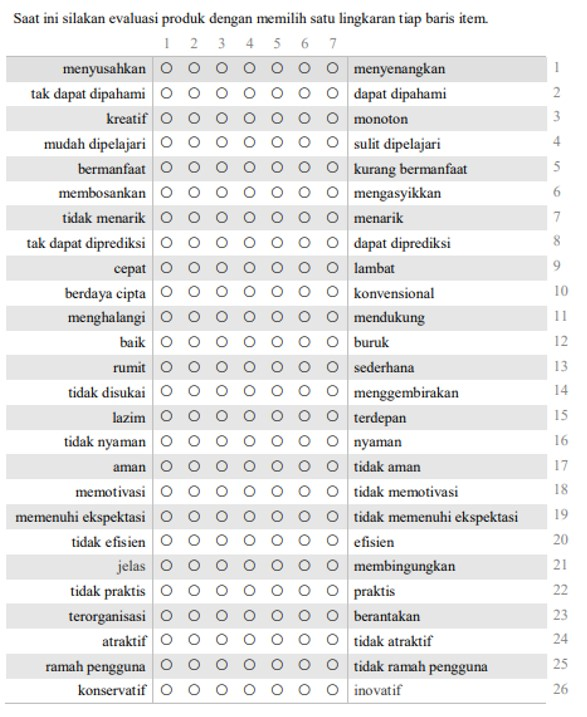
\includegraphics[width=0.6\textwidth]{assets/gambar3.jpg}
    \\\textbf{Gambar 3. Rancangan Database}
\end{center}

\noindent\hspace{1cm}Penelitian ini diawali dengan studi literatur untuk mempelajari landasan teori dan penelitian terdahulu yang relevan sebagai dasar dalam merancang metode dan analisis. Subjek penelitian adalah masyarakat umum di Kabupaten Subang yang menggunakan platform pembayaran digital seperti GoPay, OVO, dan DANA \cite{1}.

\noindent\hspace{1cm}Untuk mengukur pengalaman pengguna, penelitian ini menggunakan dua alat evaluasi yaitu \textit{System Usability Scale (SUS)} dan \textit{User Experience Questionnaire (UEQ)}. Proses berikut dilakukan dalam penelitian:

\begin{enumerate}[leftmargin=2em]
    \item \textbf{Penentuan Parameter Kuesioner}

    \noindent\hspace{1cm}\textit{System Usability Scale (SUS)}: Kuesioner terdiri dari 10 pertanyaan dengan 5 pilihan jawaban yang berkisar dari "Sangat Tidak Setuju" hingga "Sangat Setuju." Skor SUS dihitung berdasarkan jawaban responden, dengan nilai minimum 0 dan maksimum 100. Metode perhitungan melibatkan penjumlahan total nilai jawaban yang kemudian diolah menggunakan rumus standar SUS untuk menghasilkan skor akhir \cite{11}.

    \noindent\hspace{1cm}\textit{User Experience Questionnaire (UEQ)}: Parameter dalam kuesioner ini dirancang untuk mengevaluasi enam dimensi pengalaman pengguna, yaitu \textit{Daya Tarik, Kejelasan, Efisiensi, Keandalan, Stimulasi}, dan \textit{Kebaruan}. Masing-masing dimensi dinilai melalui skala semantik diferensial dengan rentang skor dari -3 hingga +3.

    \item \textbf{Pengumpulan Data}

    \noindent\hspace{1cm}Responden diminta untuk mengisi kuesioner SUS dan UEQ setelah menggunakan platform pembayaran digital. Data yang dikumpulkan meliputi skor kuantitatif dari kedua kuesioner \cite{12}.

    \item \textbf{Analisis Data}

    \noindent\hspace{1cm}\textit{System Usability Scale (SUS)}: Skor dari kuesioner dianalisis menggunakan statistik deskriptif untuk menentukan tingkat kegunaan (\textit{usability}). Skor SUS diinterpretasikan dengan panduan standar, di mana nilai di atas 68 menunjukkan kegunaan yang baik \cite{14}.

    \noindent\hspace{1cm}\textit{User Experience Questionnaire (UEQ)}: Data dari kuesioner UEQ dianalisis untuk menghitung skor rata-rata pada setiap dimensi pengalaman pengguna. Hasilnya dibandingkan dengan \textit{benchmark} UEQ untuk menilai kualitas pengalaman pengguna relatif terhadap produk lain \cite{15}.
\end{enumerate}
% ----- Foto
\begin{center}
    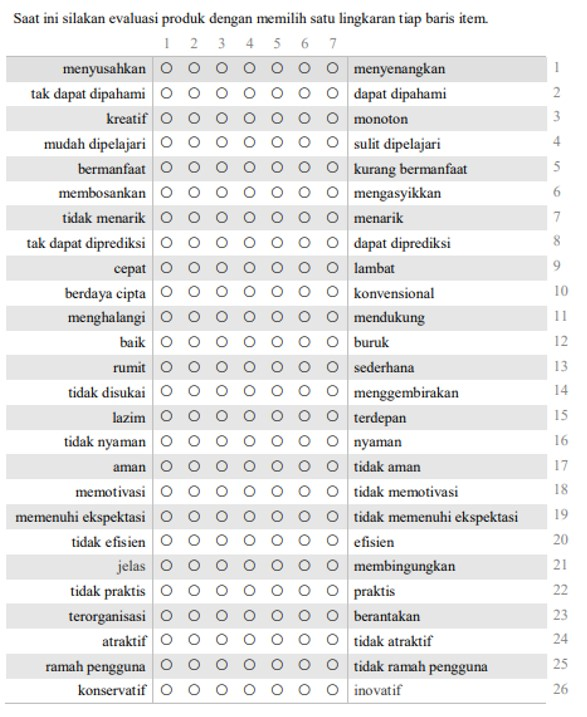
\includegraphics[width=0.6\textwidth]{assets/gambar3.jpg}
    \\\textbf{Gambar 3. Rancangan Database}
\end{center}

Sedangkan pada kuesioner UEQ menggunakan 26 item pernyataan yang berasal dari 6 aspek skala, yaitu: Daya tarik merupakan kesan dari produk, apakah responden menyukai atau tidak saat menggunakan produk tersebut. Kejelasan merupakan kesan responden untuk mengukur apakah responden mudah mengenal sebuah produk, efisiensi merupakan kesan yang tentang apakah responden bisa menggunakan produk secara efisien dan cepat. Ketepatan merupakan kesan berupa apakah responden bisa mengendalikan interaksi pada sebuah produk, stimulasi merupakan kesan responden apakah tertarik atau termotivasi dalam menggunakan sebuah produk dan kebaruan merupakan kesan dari produk apakah ada sifat inovatif dan kreatif serta apakah bisa menarik perhatian responden dalam menggunakan sebuah produk. Berikut adalah daftar item pernyataan kuesioner UEQ: 

% ----- Foto
\begin{center}
    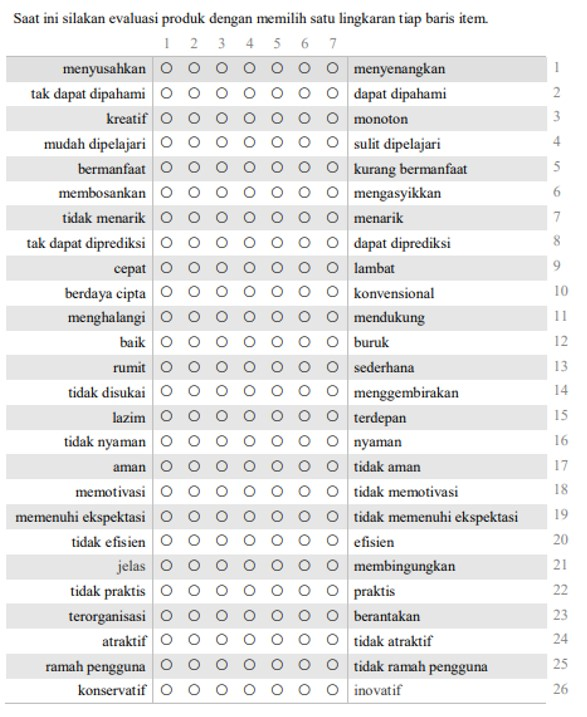
\includegraphics[width=0.6\textwidth]{assets/gambar3.jpg}
    \\\textbf{Gambar 3. Rancangan Database}
\end{center}


Langkah berikutnya adalah penentuan responden kuesioner sus dan kuesioner ueq. Pada kuesioner sus, menurut (Nielsen, 2012) Sedangkan jumlah responden yang dibutuhkan untuk mengisi kuesioner SUS adalah 20 responden. Jumlah tersebut merupakan jumlah yang optimal untuk melakukan studi kuantitatif. Oleh sebab itu, dalam penelitian ini menggunakan 20 responden untuk studi perbandingan kuesioner sus pada aplikasi GoPay, OVO dan Dana. sedangkan responden kuesioner ueq, menurut benchmark dari ueq untuk pengukuran yang stabil cukup menggunakan 20-30 responden. Oleh sebab itu, dalam penelitian ini menggunakan 30 responden untuk kuesioner ueq \cite{5}. 
Selanjutnya dilakukan analisis dan pembahasan dari hasil pengumpulan data kuesioner SUS dan kuesioner UEQ yang telah dilakukan sebelumnya. Pada tahapan ini akan dijabarkan hasil dari kuesioner SUS dan hasil dari kuesioner UEQ. Selanjutnya akan dilakukan perbandingan dari hasil kuesioner SUS dan kuesioner UEQ pada ketiga aplikasi. Pengambilan kesimpulan dilakukan setelah semua tahapan-tahapan dalam penelitian selesai dilakukan\cite{13}.

%%%%%%%%%%%%%%%%%%%%%%%%%%%%%%%%%%%%%%%%%% HASIL %%%%%%%%%%%%%%%%%%%%%%%%%%%%
\section{Hasil}
%%%%%%%%%%%%%%%%%%%%%%%%%%%%%%%%%%%%%PEMBAHASAN %%%%%%%%%%%%%%%%%%%%%

\subsection{System Usability Scale (SUS)}

\section{Hasil}

Hasil kuesioner \textit{System Usability Scale (SUS)} pada aplikasi GoPay dapat dilihat pada Tabel~\ref{tab:sus_gopay} berikut:
\usepackage{graphicx}

% ----- Tabel 1 
\begin{table}[hbt!]
    \begin{threeparttable}
        \begin{tabular}{l*{10}{c}}
            \toprule
            \textbf{NO} & \textbf{R1} & \textbf{R2} & \textbf{R3} & \textbf{R4} & \textbf{R5} & \textbf{R6} & \textbf{R7} & \textbf{R8} & \textbf{R9} & \textbf{R10} \\
            \midrule
            1  & 2 & 3 & 3 & 4 & 2 & 2 & 3 & 3 & 3 & 3 \\
            \hline
            2  & 4 & 3 & 3 & 3 & 2 & 2 & 0 & 3 & 3 & 3 \\
            \hline
            3  & 3 & 4 & 3 & 4 & 2 & 1 & 0 & 3 & 3 & 1 \\
            \hline
            4  & 1 & 1 & 1 & 1 & 1 & 1 & 1 & 1 & 1 & 2 \\
            \hline
            5  & 0 & 2 & 3 & 3 & 3 & 0 & 2 & 1 & 1 & 0 \\
            \hline
            6  & 2 & 3 & 3 & 2 & 0 & 0 & 4 & 4 & 1 & 1 \\
            \hline
            7  & 2 & 1 & 1 & 1 & 2 & 0 & 1 & 2 & 0 & 1 \\
            \hline
            8  & 1 & 1 & 0 & 2 & 4 & 3 & 2 & 2 & 3 & 0 \\
            \hline
            9  & 4 & 3 & 3 & 3 & 4 & 4 & 2 & 2 & 1 & 1 \\
            \hline
            10 & 3 & 3 & 4 & 3 & 1 & 1 & 2 & 1 & 1 & 0 \\
            \hline
            11 & 2 & 3 & 3 & 1 & 0 & 0 & 2 & 2 & 3 & 3 \\
            \hline
            12 & 1 & 1 & 0 & 2 & 1 & 4 & 3 & 2 & 3 & 0 \\
            \hline
            13 & 1 & 1 & 1 & 2 & 1 & 2 & 3 & 3 & 1 & 4 \\
            \hline
            14 & 1 & 1 & 0 & 0 & 1 & 0 & 2 & 4 & 3 & 2 \\
            \hline
            15 & 3 & 1 & 2 & 4 & 4 & 3 & 2 & 3 & 3 & 2 \\
            \hline
            16 & 0 & 0 & 1 & 1 & 1 & 2 & 1 & 4 & 3 & 2 \\
            \hline
            17 & 1 & 2 & 1 & 2 & 2 & 3 & 3 & 3 & 4 & 1 \\
            \hline
            18 & 1 & 1 & 1 & 1 & 2 & 3 & 3 & 3 & 1 & 4 \\
            \hline
            19 & 0 & 3 & 4 & 2 & 4 & 3 & 3 & 1 & 2 & 3 \\
            \hline
            20 & 3 & 3 & 3 & 2 & 1 & 1 & 1 & 2 & 2 & 4 \\
            \midrule
            \textbf{Total Skor}   & 35 & 40 & 40 & 43 & 38 & 35 & 40 & 47 & 42 & 37 \\
            \hline
            \textbf{Skor x 2.5}   & 87.5 & 100 & 100 & 107.5 & 95 & 87.5 & 100 & 117.5 & 105 & 92.5 \\
            \bottomrule
        \end{tabular}
        \caption{Perhitungan System Usability Scale (SUS) GoPay}
        \label{tabel:sus_gopay}
    \end{threeparttable}
\end{table}

Kemudian, nilai akhir rata-rata dari skor SUS dihitung dengan menjumlahkan seluruh skor hasil akhir dan membaginya dengan jumlah responden: \\ \\ 
\text{Rata-rata} 
\[
\frac{87.5 + 100 + 100 + 107.5 + 95 + 87.5 + 100 + 117.5 + 105 + 92.5}{10} = 99.75
\]

\textbf{= 50} \\ \\ 
Menghitung nilai akhir rata-rata dari skor SUS dengan menjumlahkan hasil akhir semua responden dan membaginya dengan jumlah responden. Hasil analisis perhitungan aplikasi GoPay mendapatkan nilai sebesar 50 dengan grade F, peringkat OK, dan kategori low berdasarkan interpretasi SUS score dari jurnal yang ditulis oleh Sidik \cite{9}.

% ----- Tabel 2
\begin{table}[hbt!]
    \begin{threeparttable}
        \caption{Perhitungan System Usability Scale (SUS) OVO}
        \label{tabel:sus_ovo}
        \begin{tabular}{l*{10}{c}}
            \toprule
            \textbf{NO} & \textbf{R1} & \textbf{R2} & \textbf{R3} & \textbf{R4} & \textbf{R5} & \textbf{R6} & \textbf{R7} & \textbf{R8} & \textbf{R9} & \textbf{R10} \\
            \midrule
            1  & 0 & 0 & 1 & 2 & 0 & 1 & 2 & 2 & 4 & 3 \\
            \hline
            2  & 3 & 2 & 1 & 1 & 2 & 3 & 3 & 0 & 2 & 3 \\
            \hline
            3  & 2 & 1 & 1 & 0 & 1 & 4 & 3 & 0 & 2 & 1 \\
            \hline
            4  & 1 & 1 & 4 & 3 & 0 & 2 & 2 & 1 & 1 & 0 \\
            \hline
            5  & 2 & 3 & 4 & 4 & 4 & 1 & 0 & 3 & 0 & 1 \\
            \hline
            6  & 1 & 1 & 1 & 0 & 0 & 4 & 2 & 3 & 0 & 1 \\
            \hline
            7  & 1 & 1 & 0 & 1 & 3 & 3 & 0 & 0 & 2 & 2 \\
            \hline
            8  & 3 & 4 & 1 & 0 & 2 & 2 & 1 & 0 & 1 & 4 \\
            \hline
            9  & 4 & 3 & 4 & 3 & 1 & 1 & 4 & 4 & 1 & 2 \\
            \hline
            10 & 1 & 2 & 0 & 3 & 3 & 3 & 4 & 4 & 2 & 3 \\
            \hline
            11 & 4 & 3 & 1 & 2 & 0 & 0 & 1 & 1 & 2 & 1 \\
            \hline
            12 & 1 & 2 & 3 & 3 & 3 & 3 & 3 & 4 & 4 & 3 \\
            \hline
            13 & 4 & 3 & 2 & 1 & 0 & 3 & 2 & 1 & 0 & 4 \\
            \hline
            14 & 4 & 0 & 2 & 0 & 3 & 4 & 4 & 2 & 1 & 1 \\
            \hline
            15 & 3 & 3 & 3 & 1 & 1 & 0 & 1 & 1 & 4 & 3 \\
            \hline
            16 & 0 & 3 & 4 & 0 & 1 & 2 & 2 & 4 & 2 & 3 \\
            \hline
            17 & 0 & 4 & 3 & 3 & 4 & 1 & 2 & 2 & 1 & 2 \\
            \hline
            18 & 3 & 3 & 0 & 1 & 1 & 1 & 4 & 3 & 1 & 4 \\
            \hline
            19 & 3 & 3 & 3 & 2 & 4 & 3 & 0 & 0 & 3 & 2 \\
            \hline
            20 & 1 & 2 & 4 & 2 & 0 & 1 & 4 & 1 & 1 & 3 \\
            \midrule
            \textbf{Total Skor}   & 41 & 44 & 42 & 32 & 33 & 42 & 44 & 36 & 34 & 46 \\
            \hline
            \textbf{Skor x 2.5}   & 102.5 & 110 & 105 & 80 & 82.5 & 105 & 110 & 90 & 85 & 115 \\
            \bottomrule
        \end{tabular}
    \end{threeparttable}
\end{table}

Kemudian menghitung nilai akhir rata-rata dari skor SUS dengan menjumlahkan hasil akhir semua responden dan membaginya dengan jumlah responden.
\text{Rata-rata} 
\[
\text{Rata-rata} = \frac{102.5 + 110 + 105 + 80 + 82.5 + 105 + 110 + 90 + 85 + 115}{10} = 98.5
\]

\textbf{= 49}
Menghitung nilai akhir rata-rata dari skor SUS dengan menjumlahkan hasil akhir semua responden dan membaginya dengan jumlah responden. Hasil analisis perhitungan aplikasi OVO mendapatkan nilai sebesar 49 dengan grade F, peringkat OK, dan kategori low berdasarkan interpretasi SUS score dari jurnal yang ditulis oleh Sidik \cite{9}.
% ----- Tabel 3
\usepackage{float} % Pastikan ini ada di preamble

\begin{table}[H]
    \begin{threeparttable}
        \caption{Perhitungan System Usability Scale (SUS) DANA}
        \label{tabel:sus_dana}
        \begin{tabular}{l*{10}{c}}
            \toprule
            \textbf{NO} & \textbf{R1} & \textbf{R2} & \textbf{R3} & \textbf{R4} & \textbf{R5} & \textbf{R6} & \textbf{R7} & \textbf{R8} & \textbf{R9} & \textbf{R10} \\
            \midrule
            1  & 4 & 3 & 3 & 2 & 4 & 4 & 1 & 3 & 2 & 0 \\
            2  & 3 & 2 & 1 & 0 & 1 & 2 & 0 & 4 & 2 & 1 \\
            3  & 0 & 2 & 4 & 3 & 4 & 3 & 3 & 0 & 1 & 3 \\
            4  & 2 & 0 & 1 & 0 & 0 & 3 & 2 & 1 & 2 & 3 \\
            5  & 4 & 3 & 3 & 3 & 3 & 3 & 3 & 3 & 4 & 2 \\
            6  & 1 & 4 & 4 & 2 & 3 & 1 & 1 & 4 & 2 & 1 \\
            7  & 3 & 0 & 3 & 0 & 0 & 2 & 1 & 1 & 3 & 3 \\
            8  & 2 & 1 & 1 & 1 & 2 & 4 & 1 & 1 & 4 & 4 \\
            9  & 0 & 2 & 3 & 3 & 4 & 3 & 2 & 4 & 4 & 2 \\
            10 & 4 & 0 & 1 & 1 & 4 & 1 & 1 & 4 & 2 & 1 \\
            11 & 4 & 3 & 4 & 3 & 3 & 3 & 2 & 4 & 4 & 2 \\
            12 & 3 & 2 & 1 & 1 & 2 & 0 & 1 & 1 & 1 & 0 \\
            13 & 1 & 1 & 1 & 1 & 2 & 3 & 3 & 2 & 4 & 3 \\
            14 & 3 & 3 & 2 & 0 & 0 & 3 & 1 & 1 & 2 & 4 \\
            15 & 2 & 3 & 3 & 2 & 0 & 2 & 3 & 0 & 4 & 3 \\
            16 & 3 & 0 & 0 & 2 & 2 & 3 & 0 & 1 & 1 & 3 \\
            17 & 1 & 1 & 1 & 0 & 1 & 1 & 1 & 4 & 2 & 2 \\
            18 & 4 & 3 & 3 & 2 & 4 & 3 & 2 & 3 & 3 & 1 \\
            19 & 1 & 1 & 1 & 1 & 2 & 4 & 0 & 2 & 3 & 3 \\
            20 & 4 & 4 & 4 & 3 & 3 & 2 & 0 & 2 & 3 & 2 \\
            \midrule
            \textbf{Total Skor}   & 49 & 38 & 44 & 30 & 44 & 50 & 28 & 45 & 53 & 43 \\
            \textbf{Skor x 2.5}   & 122.5 & 95 & 110 & 75 & 110 & 125 & 70 & 112.5 & 132.5 & 107.5 \\
            \bottomrule
        \end{tabular}
    \end{threeparttable}
\end{table}
\text{Rata-rata} 
\[
\text{Rata-rata} = \frac{122.5 + 95 + 110 + 75 + 110 + 125 + 70 + 112.5 + 132.5 + 107.5}{10} = 106
\]
\textbf{= 53}
Menghitung nilai akhir rata-rata dari skor SUS dengan menjumlahkan hasil akhir semua responden dan membaginya dengan jumlah responden. Hasil analisis perhitungan aplikasi Dana mendapatkan nilai sebesar 53 dengan grade F, peringkat Good, dan kategori low berdasarkan interpretasi SUS score dari jurnal yang ditulis oleh Sidik \cite{9}.


% \clearpage
\subsection{User Experience Questionnaire (UEQ)}
%  ----- p1
Hasil kuesioner UEQ pada aplikasi GoPay, OVO dan Dana dapat dilihat pada Gambar 4, Gambar 5 dan Gambar 6 berikut:
% ----- Foto
\begin{center}
    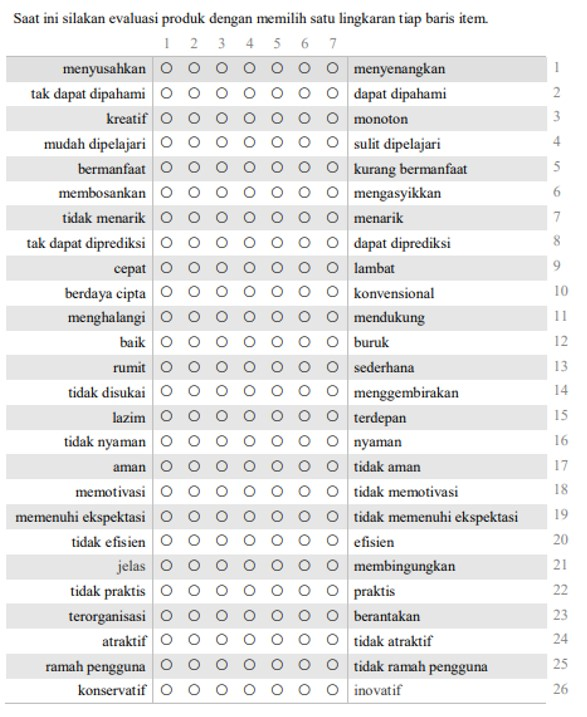
\includegraphics[width=0.6\textwidth]{assets/gambar3.jpg}
    \\\textbf{Gambar 3. Rancangan Database}
\end{center}



% ----- p2
Berdasarkan Gambar  bisa disimpulkan bahwa aplikasi GoPay cenderung memiliki kesan yang baik terhadap responden pada saat menggunakan aplikasi GoPay. Hal ini dikarenakan terdapat enam aspek yang mendapatkan nilai rata-rata berkisar antara -0,8 dan 0,8 atau berada pada level normal yang ditandai dengan area berwarna kuning. Urutan aspek dari nilai rata-rata tertinggi ke terendah yaitu Efisiensi, Kejelasan, Daya tarik, Ketepatan, Stimulasi dan Kebaruan.
% ----- Foto
\begin{center}
    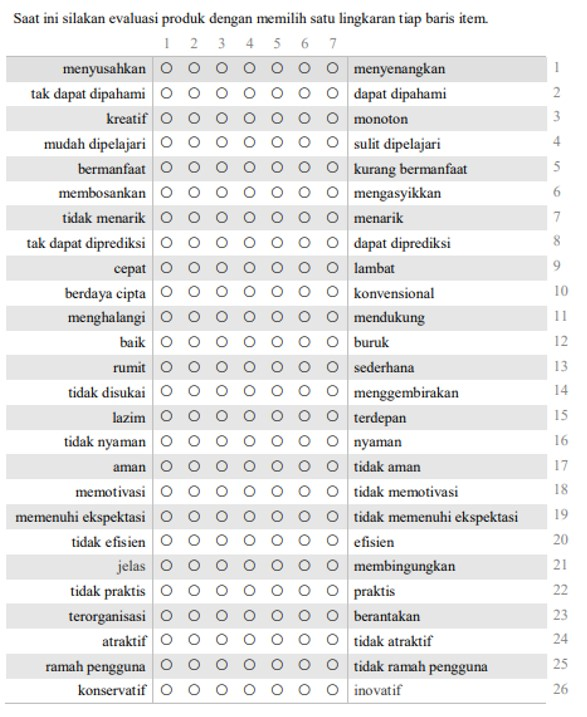
\includegraphics[width=0.6\textwidth]{assets/gambar3.jpg}
    \\\textbf{Gambar 3. Rancangan Database}
\end{center}

% ----- p3
Berdasarkan Gambar  bisa disimpulkan bahwa aplikasi OVO cenderung memiliki kesan yang cukup baik terhadap responden pada saat menggunakan aplikasi OVO. Hal ini dikarenakan terdapat empat aspek yang mendapatkan nilai rata-rata berkisar antara -0,8 dan 0,8 atau berada pada level normal yang ditandai dengan area berwarna kuning. Sedangkan dua aspek yang mendapatkan nilai rata-rata berkisar antara -0,8 berada pada level negatif. Urutan aspek dari nilai rata-rata tertinggi ke terendah yaitu Efisiensi, Daya tarik, Kejelasan, Ketepatan, Kebaruan dan Stimulasi. 
% ----- Foto
\begin{center}
    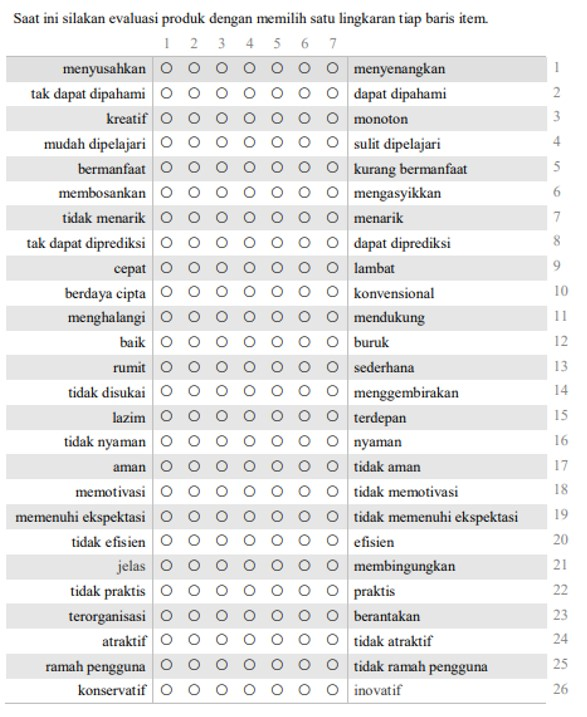
\includegraphics[width=0.6\textwidth]{assets/gambar3.jpg}
    \\\textbf{Gambar 3. Rancangan Database}
\end{center}


% ----- p4
Berdasarkan Gambar  bisa disimpulkan bahwa aplikasi Dana cenderung memiliki kesan yang baik terhadap responden pada saat menggunakan aplikasi Dana. Hal ini dikarenakan terdapat enam aspek yang mendapatkan nilai rata-rata berkisar antara -0,8 dan 0,8 atau berada pada level normal yang ditandai dengan area berwarna kuning. Urutan aspek dari nilai rata-rata tertinggi ke terendah yaitu Daya tarik, Kejelasan, Kebaruan, Efisiensi, Stimulasi dan Ketepatan.
% ----- Foto
\begin{center}
    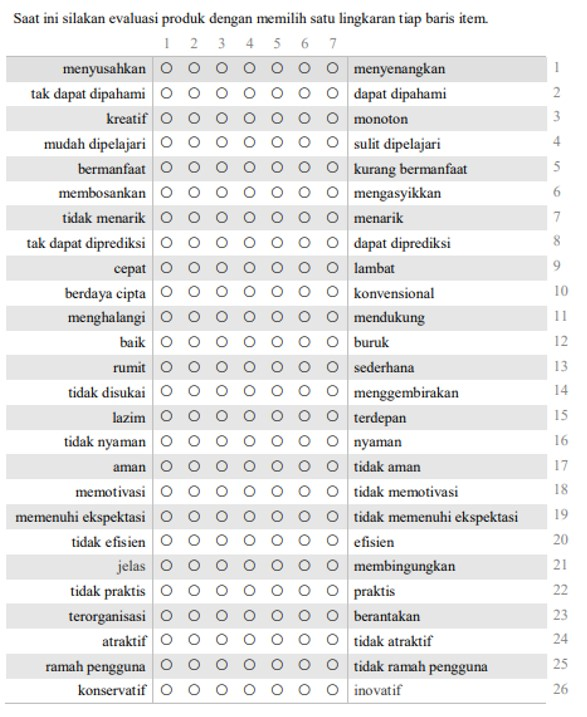
\includegraphics[width=0.6\textwidth]{assets/gambar3.jpg}
    \\\textbf{Gambar 3. Rancangan Database}
\end{center}

% \clearpage
% ----- p1
\subsection{Perbandingan System Usability Scale (SUS) dan User Experience Questionnaire (UEQ)}
Hasil System Usability Scale (SUS) terhadap ketiga aplikasi dirangkum dalam Gambar 7: 
% ----- Foto
\begin{center}
    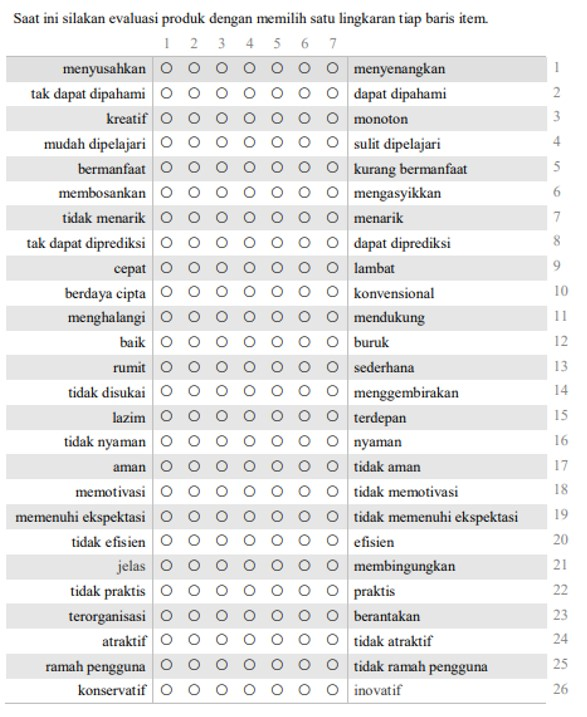
\includegraphics[width=0.6\textwidth]{assets/gambar3.jpg}
    \\\textbf{Gambar 3. Rancangan Database}
\end{center}


% -----p5
Perbandingan hasil kuesioner SUS menunjukkan aplikasi Dana mendapatkan hasil lebih baik atau lebih tinggi daripada hasil dari aplikasi GoPay dan OVO. Hasil analisis perhitungan aplikasi GoPay mendapatkan nilai sebesar 50 dengan grade F, peringkat OK, dan kategori low, hasil analisis perhitungan aplikasi OVO mendapatkan nilai sebesar 49 dengan grade F, peringkat OK, dan kategori low serta hasil analisis perhitungan aplikasi Dana mendapatkan nilai sebesar 53 dengan grade F, peringkat OK, dan kategori Good. Dikarenakan 3 aplikasi tersebut sama-sama mendapatkan grade F dan kategori Low, Tetapi aplikasi Dana memiliki hasil lebih tinggi yaitu dengan skor 53 dan peringkat Good.

% ----- Foto
\begin{center}
    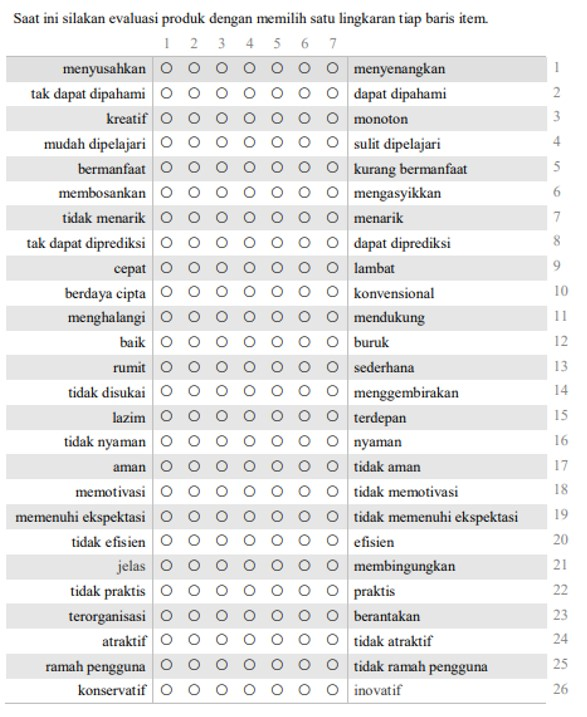
\includegraphics[width=0.6\textwidth]{assets/gambar3.jpg}
    \\\textbf{Gambar 3. Rancangan Database}
\end{center}


% ----- p 6-1
Berdasarkan hasil kuesioner UEQ dapat diketahui nilai rata-rata dari masing-masing aspek skala UEQ. Pada aspek skala Daya tarik aplikasi GoPay mendapat nilai rata-rata lebih baik dengan nilai 0,539, nilai rata-rata aplikasi OVO mendapatkan nilai 0,111 dan nilai rata-rata aplikasi Dana 0,517. Pada aspek skala Kejelasan aplikasi GoPay mendapat nilai rata-rata lebih baik dengan nilai 0,692, nilai rata-rata aplikasi OVO mendapatkan nilai 0,108 dan nilai rata-rata aplikasi Dana 0,500. 
 \\ \\ 
% ----- p 6-
Pada aspek skala Efisiensi aplikasi GoPay mendapat nilai rata-rata lebih baik sebesar 0,725, nilai rata-rata aplikasi OVO mendapatkan nilai 0,442 dan nilai rata-rata aplikasi Dana 0,417. Pada aspek skala Ketepatan aplikasi GoPay mendapat nilai rata-rata lebih baik dengan nilai sebesar 0,517, nilai rata-rata aplikasi OVO mendapatkan nilai 0,100 dan nilai rata-rata aplikasi Dana 0,300. Pada aspek skala Stimulasi aplikasi GoPay mendapatkan nilai rata-rata lebih baik dengan nilai 1,513, sedangkan nilai rata-rata aplikasi Dana mendapat nilai sebesar 0,483. Sedangkan aspek skala Kebaruan pada aplikasi Dana mendapatkan nilai rata-rata lebih baik dengan nilai sebesar 0,483 dibandingkan dengan aplikasi GoPay yang mendapatkan nilai rata-rata sebesar 0,300. 

% ----- p 6-3
Berdasarkan pada Gambar 8, perbandingan hasil kuesioner UEQ menunjukkan aplikasi GoPay mendapatkan hasil lebih baik atau lebih tinggi daripada hasil dari aplikasi OVO dan aplikasi Dana. dikarenakan aplikasi GoPay memiliki hasil lebih tinggi pada lima aspek yaitu Daya tarik, Kejelasan, Efisiensi, Ketepatan dan Stimulasi, sedangkan aplikasi Dana mendapatkan hasil lebih baik dalam satu aspek skala yaitu aspek Kebaruan.

%%%%%%%%%%%%%%%%%%%%%%%%%%%%%%%%%%% SIMPULAN %%%%%%%%%%%%%%%%%%%%%%%%%
% \clearpage
\section{Simpulan}

Berdasarkan pembahasan mengenai perbandingan pengujian tentang pengalaman pengguna aplikasi pembayaran digital GoPay, OVO dan Dana dengan populasi yang diambil dari masyarakat umum pengguna aplikasi GoPay, OVO dan Dana di wilayah Kabupaten Subang. Maka dapat disimpulkan hasil analisis dengan pengujian System Usability Scale (SUS) menunjukkan aplikasi Dana mendapatkan nilai sebesar 53, sedangkan aplikasi GoPay mendapatkan nilai sebesar 50 dan aplikasi OVO mendapatkan nilai 49. Selanjutnya, hasil analisis dengan pengujian User Experience Questionnaire (UEQ) menunjukan bahwa aplikasi GoPay unggul dalam lima aspek yaitu Daya tarik, Kejelasan, Efisiensi, Ketepatan dan Stimulasi, sedangkan aplikasi Dana mendapatkan hasil lebih baik dalam satu aspek skala yaitu aspek Kebaruan. Hasil pengujian perbandingan ketiga aplikasi pembayaran digital menunjukkan bahwa faktor monoton dan konvensional memiliki impresi yang normal dan di bawah rata-rata. Untuk meningkatkan nilai ini, perlu diupayakan desain aplikasi yang lebih kreatif dan inovatif.


%%%%%%%%%%%%%%%%%%%%%%%%%%%%%%%%%%% PUSTAKA %%%%%%%%%%%%%%%%%%%%%%%%%%%%%%%

\renewcommand{\refname}{Pustaka} %%% nonaktifkan bila artikel bahasa inggris
	\bibliographystyle{IEEEtran}
\bibliography{reference}

%run it with pdflatex <file>, biber <file>, pdflatex <file>
%  --------------------- Manual daftar pustaka ---------------------
%\end{CJK*}
\end{document}
